%!TEX root = ../../Main.tex
\graphicspath{{Chapters/Observer/}}
%-------------------------------------------------------------------------------

\section{Observer}
I tidligere afsnit har vi beskrevet hvordan vi har designet vores controller. Men designet af en controller afhænger af at vi har adgang til state variablerne, så vi gennem feedback kan tillægge de ønskede forstærkninger. Måden hvorpå vi fik adgang til vores state variabler i sidste afsnit, vil give os et problem når vi ønsker at implementere vores controller på det virkelige system. På \autoref{fig:cl_system_makeret_plant} kan man se, hvordan vi hiver state variablerne ud direkte inde fra systemet, som er omridset med rød. Dette er ikke muligt på et virkeligt system.

\begin{figure}[H]
	\centering
	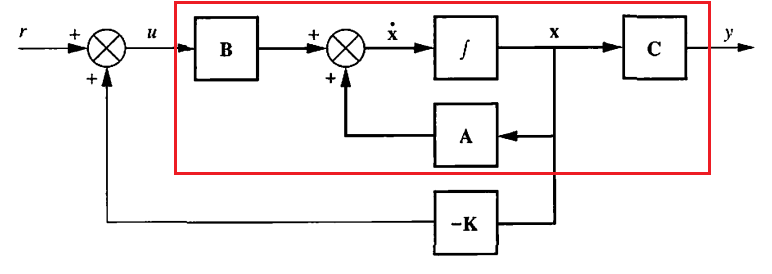
\includegraphics[width = 300pt]{Img/cl_system_makeret_plant.PNG}
	\caption{State space block diagram uden D}
	\label{fig:cl_system_makeret_plant}
\end{figure}


Det er her, vores observer design kommer ind i billedet. For hvis ikke det er mulig at tilgå de aktuelle states, grundet f.eks. omkostninger eller opbygningen af systemet. Er det i stedet muligt at estimere de aktuelle states via et observer design. Det er så disse estimerede states, frem for de aktuelle states, der bliver videregivet til controlleren.\\
På \autoref{eq:Observer_stateSpace_AogB} og \autoref{eq:Observer_stateSpace_C} kan man se observereren som model af systemet. Hvis vi sammenligner denne model med den faktiske model af systemet, ved at lave en subtraktion, som ses i  \autoref{eq:Subtraktion_A} og \autoref{eq:Subtraktion_C}. Her bliver det tydeligt at forskellen mellem modellerne afhænger af forskellen på den faktiske state og den estimerede state. 
\begin{equation}
\dot{\hat{x}} = A * \hat{x} + B * u
\label{eq:Observer_stateSpace_AogB}
\end{equation}

\begin{equation}
\hat{y} = C * \hat{x}
\label{eq:Observer_stateSpace_C}
\end{equation}

\begin{equation}
\dot{x} - \dot{\hat{x}} = A * (x -\hat{x})
\label{eq:Subtraktion_A}
\end{equation}

\begin{equation}
y -\hat{y} = C * (x - \hat{x})
\label{eq:Subtraktion_C}
\end{equation}

Derfor er det vigtigt, at vores estimerede state altid bliver beregnet meget hurtigere end den faktiske state. For at øge hastigheden for konvergensen mellem den faktiske og estimerede state bruger vi et feedback og sammenligner de to outputs se \autoref{fig:Observer_block_diagram} . Fejlen mellem disse to outputs fører vi så tilbage til det afledte af observeres state. På den måde vil systemet forsøge at tvinge denne fejl til 0. Med dette feedback kan vi designe et transient respons som er meget hurtigere det fra det faktiske system. 

\begin{figure}[H]
	\centering
	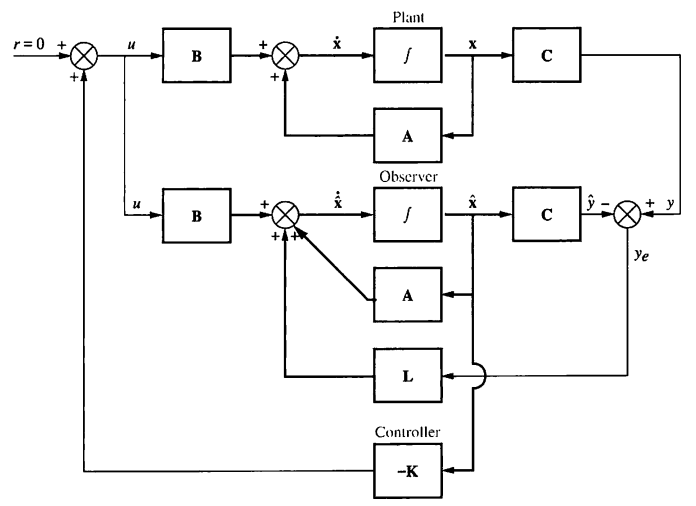
\includegraphics[width = 300pt]{Img/Observer_block_diagram.png}
	\caption{Block diagram af systemet med observer og controller}
	\label{fig:Observer_block_diagram}
\end{figure}

Lige som da vi designede controller vektor, K, består vores observer design også af en konstant vektor, L. Denne vektor, L, skal designes, så det transiente respons for observereren er hurtigere end responset fra controlleren. Derfor vælger vi at benytte de samme poler vi placerede for controlleren, vi flytter dem bare tilpas langt ud i det kontinuere domæne, så de bliver hurtige nok til ikke at have en betydelig indflydelse på dynamikken. I vores tilfælde virkerede det at gange polerne med 30. State ligningen for observeren efter L er implementeret kan ses på \autoref{eq:Observer_stateSpace_A_B_L} og \autoref{eq:Observer_stateSpace_C_L} . 
\begin{equation}
\dot{\hat{x}} = A * \hat{x} + B * u + L(y - \hat{y})
\label{eq:Observer_stateSpace_A_B_L}
\end{equation}

\begin{equation}
\hat{y} = C * \hat{x}
\label{eq:Observer_stateSpace_C_L}
\end{equation}

Det kan vi så omskrive til \autoref{eq:Observer_Omskrevet} og \autoref{eq:Observer_Omskrevet_u}

\begin{equation}
\dot{\hat{x}} = (A + B * K - L * C) * \hat{x} + L * y
\label{eq:Observer_Omskrevet}
\end{equation}

\begin{equation}
u =  K * \hat{x}
\label{eq:Observer_Omskrevet_u}
\end{equation}

Det er \autoref{eq:Observer_Omskrevet} og \autoref{eq:Observer_Omskrevet_u} vi implementere i vores system. Denne implementering skete i Simulink og kan ses på \autoref{fig:Discrete_system_med_observer} og \autoref{fig:Discrete_Observer}. Hvor \autoref{fig:Discrete_system_med_observer} er hele systemet med controller, og den lille kasse er observeren lavet som et subsystem. \autoref{fig:Discrete_Observer} er så hvad der sker inde i maven på dette subsystem, som er vores observer.


\begin{figure}[H]
	\centering
	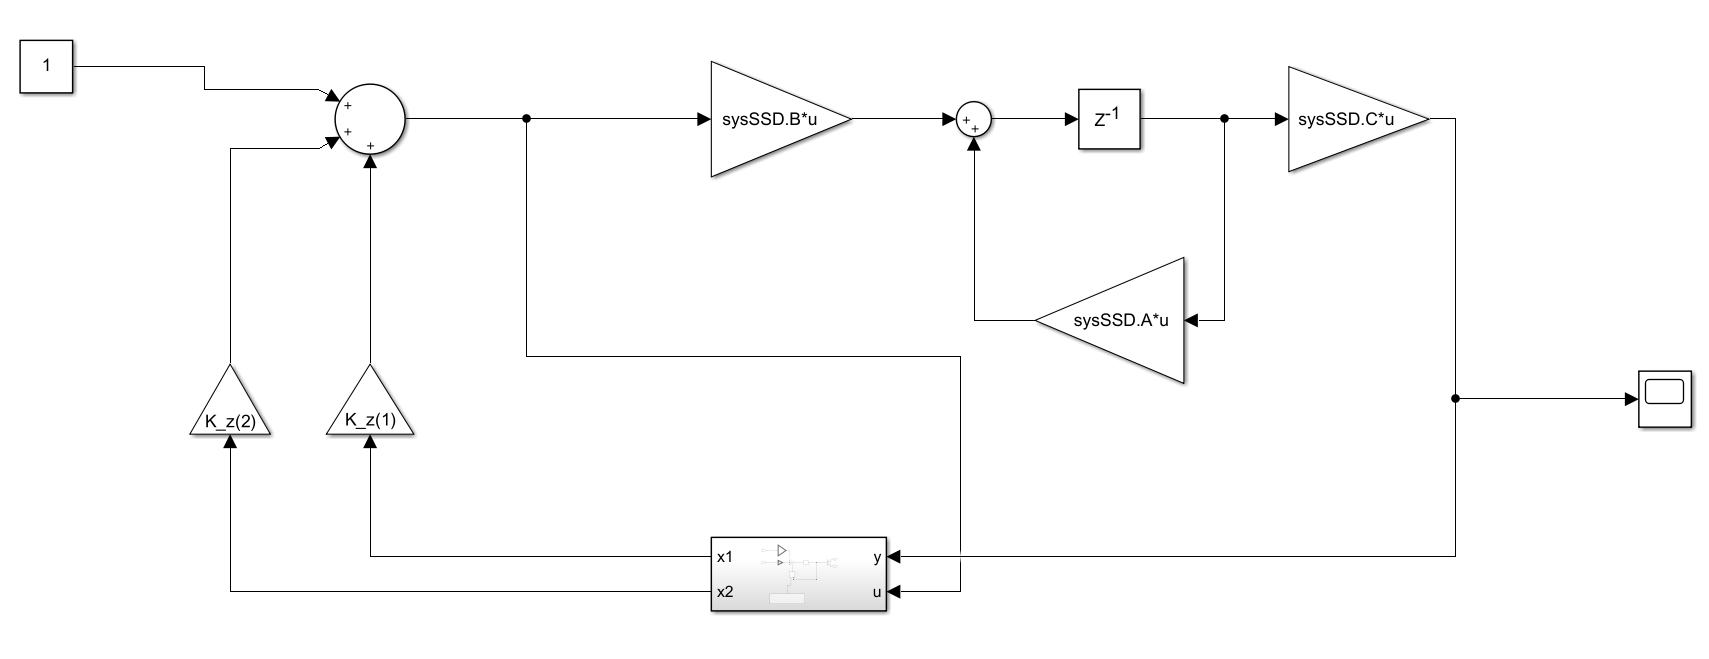
\includegraphics[width = 400pt]{Img/Discrete_system_med_observer.png}
	\caption{Block diagram af systemet med observer og controller}
	\label{fig:Discrete_system_med_observer}
\end{figure}

\begin{figure}[H]
	\centering
	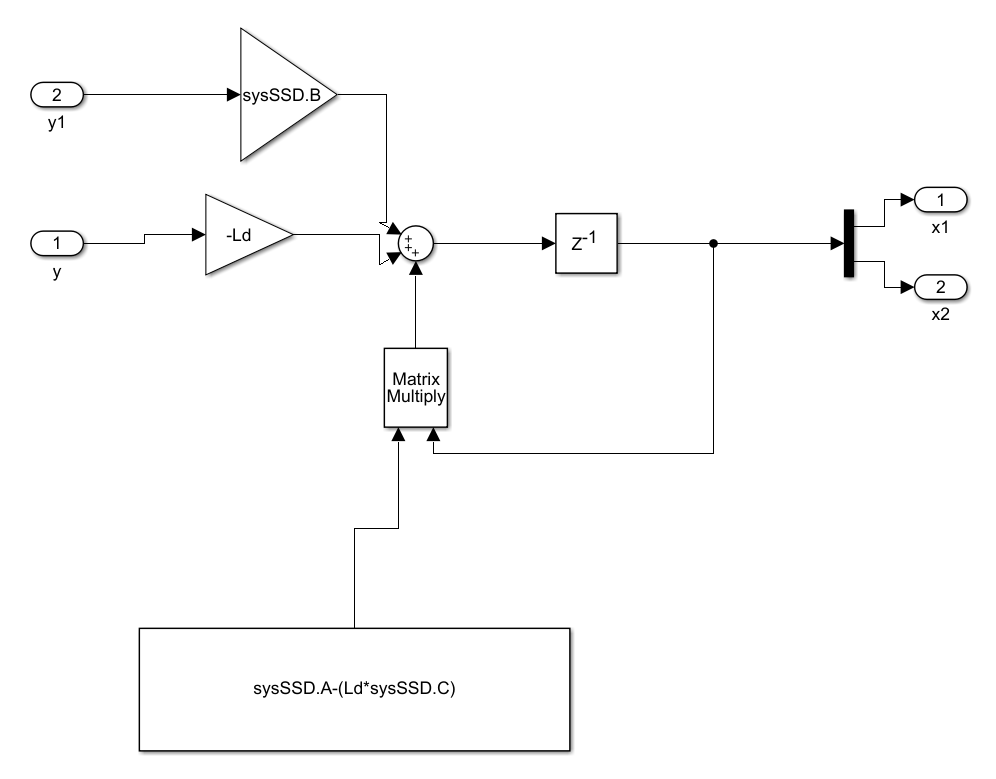
\includegraphics[width = 300pt]{Img/Discrete_Observer.png}
	\caption{Block diagram af systemet med observer og controller}
	\label{fig:Discrete_Observer}
\end{figure}

Da vi ville implementere observer designet på vores system via Simulink, skulle vi først overføre vores system til det diskrete domæne, da vores system kører digitalt. Det gjorde vi ved "c2d" functionen i matlab, som ses i den koden indsat under. Derudover har vi også benyttet os af "pole" functionen som giver polerne ud, samt "place" funktionen som giver en vektor konstant.

\begin{lstlisting}
%% Oberserver design in discrete form
sysSSD=c2d(sysSS,ts,'zoh');%Discrete

ch_eqnD = wn^2/(s^2+2*zeta*wn*s+wn^2); %Charactaristic equation
ch_eqnD = c2d(ch_eqnD,ts,'tustin');
polesD = pole(ch_eqnD);

K_z = place(sysSSD.A,sysSSD.B,polesD);
A_cl = [sysSSD.A-sysSSD.B*K_z];

sysssD_cl = ss(A_cl,sysSSD.B,sysSSD.C,sysSSD.D,ts);

observer_reqZ = polesD/30;

Ld = (place(sysSSD.A',sysSSD.C',observer_reqZ))';
\end{lstlisting}


På \autoref{Discrete_observer_simulering} kan man se simulering af vores observer design i diskret domæne. Det er tydeligt at se at vores system er stabilt, desværre har vi en markant steady state fejl, som vi ikke har kunne fjerne. Hver gang vi indsatte en ekstra pol med forstrækning, blev vores system ustabilt. Dog hvis vi sammenligner med vores closed loop opstilling uden korrigering for steady state fejl får vi meget tæt på det samme resultat. Se \autoref{Continuos_cl_simulering}. Man kan se en lille ændre, hvilket er svært at undgå da, de ektra poler der bliver tilføjet ved observeren påvirker dynamikken en smule.


\begin{figure}[H]
	\centering
	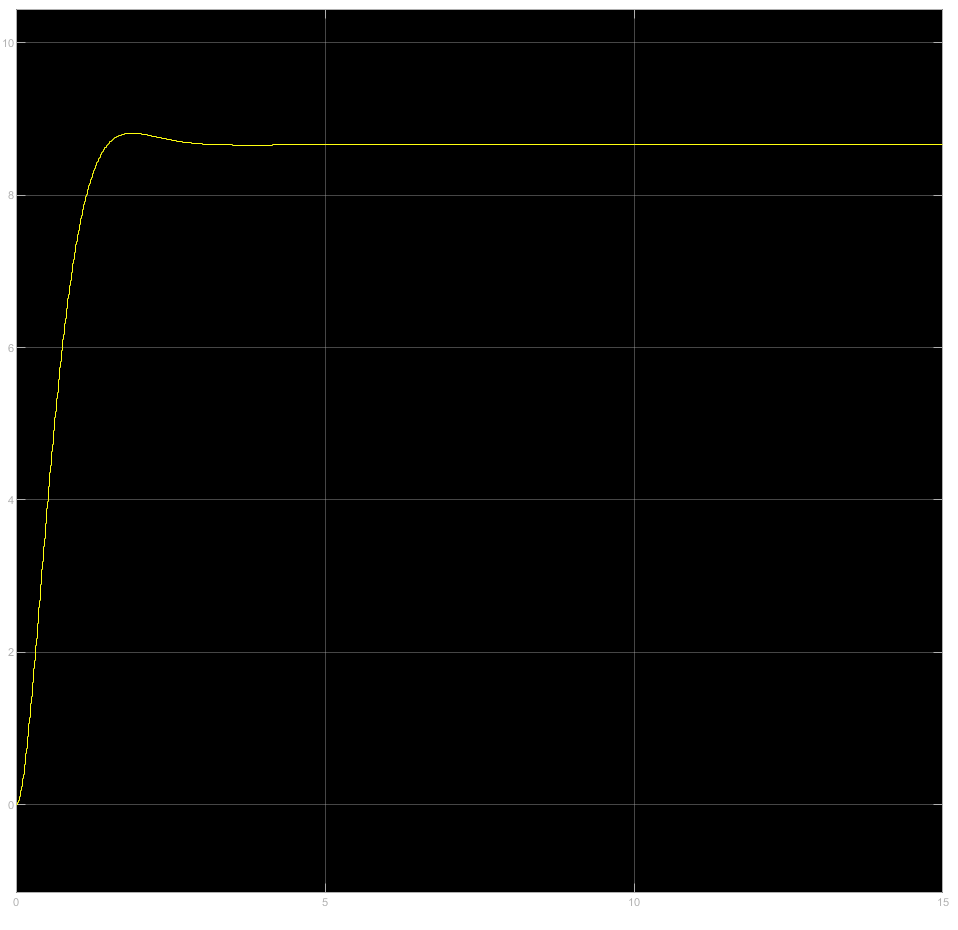
\includegraphics[width = 300pt]{Img/Discrete_observer_simulering.png}
	\caption{Block diagram af systemet med observer og controller}
	\label{Discrete_observer_simulering}
\end{figure}


\begin{figure}[H]
	\centering
	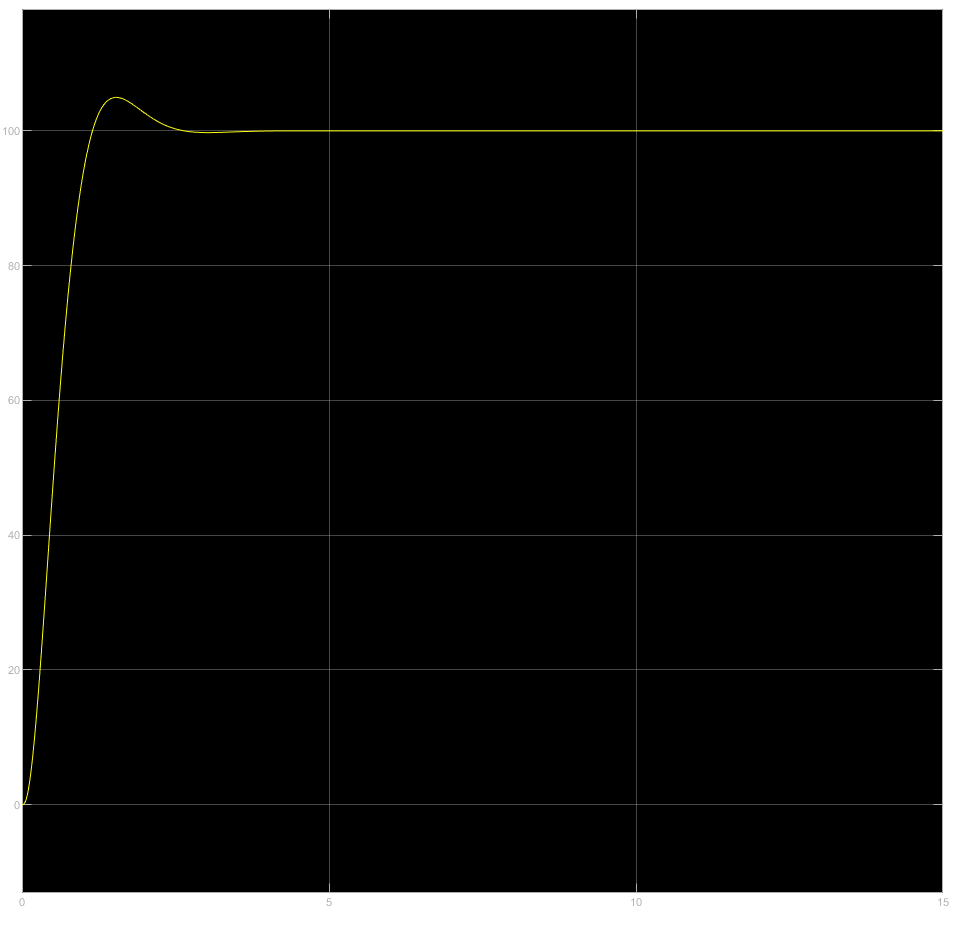
\includegraphics[width = 300pt]{Img/Continuos_cl_simulering.png}
	\caption{Block diagram af systemet med observer og controller}
	\label{Continuos_cl_simulering}
\end{figure}

Til sidst har vi så implementeret dette observer design på vores bil. Simulink opstillingen af dette kan ses på figur \autoref{Discrete_observer_paa_bil}. Bilen opførte sig helt efter forventningnen, og kørte ca 8-9 gange længere end inputet, hvilket passer med steady state fejlen. 

\begin{figure}[H]
	\centering
	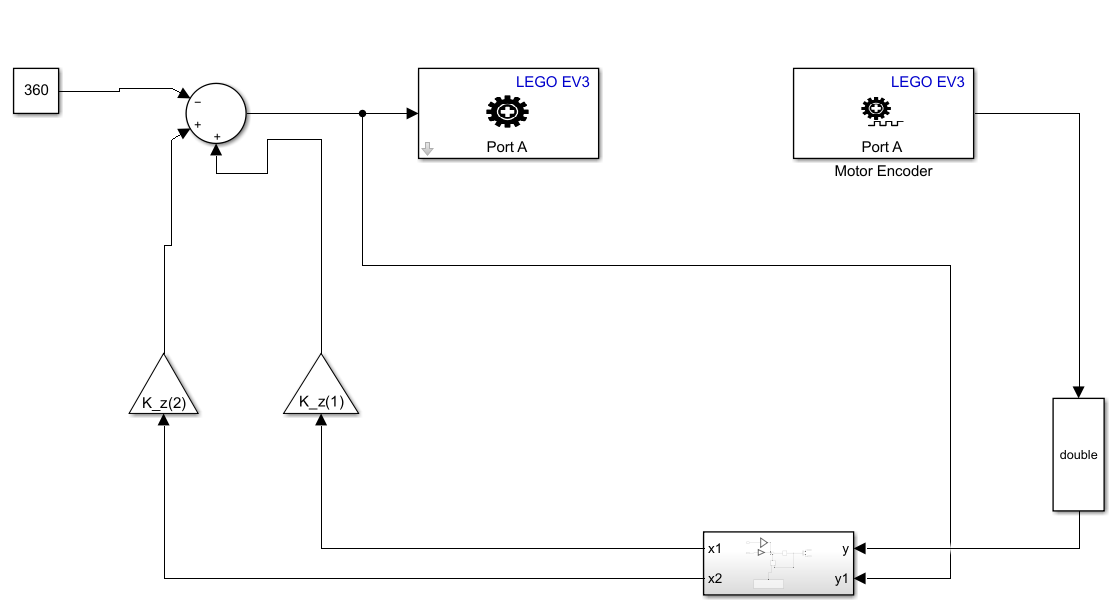
\includegraphics[width = 300pt]{Img/Discrete_observer_paa_bil.png}
	\caption{Block diagram af systemet med observer og controller}
	\label{Discrete_observer_paa_bil}
\end{figure}
